\FloatBarrier
\chapter{Building a data set for Comparative Argument Mining}
\label{sec:prestudy}
Due to the novelty of Argument Mining (and especially Comparative Argument Mining), the supply of data sets is small. Thus, a new data set had to be created.

The data set was designed to answer two questions. First, does a sentence compare two known objects? And, if it does, is the first-mentioned object better or worse than the second one? Those questions will be translated to several classification tasks in the later chapters.

The data set was created using the crowdsourcing platform CrowdFlower\footnote{https://www.crowdflower.com (23.02.2018), now called xxxxx}. As described in detail in the following chapters, the annotators were asked to assign one of four (and later three) classes to a sentence in which the objects of interest were highlighted.

% zahlen 24.03
The final data set contains 7199 sentences, each containing one of 271 object pairs. Each sentence was annotated by at least five annotators.

\section{Common Crawl Text Corpus}
The sentences for the crowdsourcing task were obtained from a CommonCrawl\footnote{https://commoncrawl.org (23.02.2018)} data set. CommonCrawl is a non-profit organisation which crawls the web and releases the crawled data for free use.

The data\footnote{Download Link} used in this thesis was already preprocessed (see \cite{Panchenko:2017aa}). First, it contains only English text. Duplicates and near-duplicates were removed, as well as all HTML tags. The texts were then split into sentences.

To make the data set managable, an ElasticSearch index was created. The index contains 3,288,963,864 unique sentences.

To get an idea if there are enough comparative sentences in the index, it was queried for all sentences containing one of the words \enquote{\emph{better}} or \enquote{\emph{worse}},  as those words often indicate a comparison. This query returns 32,946,247 matching sentences. Querying for \enquote{\emph{is better than}} still returns 428,932 sentences.

Those numbers show that there are enough sentences in the index to create a data set for the given task. Even if only 1\% of the sentences containing \enquote{\emph{is better than}} are truly comparative, there would be 4289 training examples for the machine learning algorithm using this query.


\section{Prestudies}
In preparation to the main crowdsourcing task, several questions had to be answered:
\begin{enumerate}
\item How to extract sentences from the index? (How should the query look like?)
\item How to preprocress those sentences? (How to highlight the objects of interest?)
\item Which classes should be assigned to the sentences?
\item How to phrase the guidelines?
\end{enumerate}

Two prestudies were conducted to answer those questions.



\subsection{Sentence Selection}
The sentences for the crowdsourcing task should have a high probability of being comparative so that enough positive examples for the machine learning part are present. To ensure this, a list of cue words which indicate comparison was compiled by hand. For the prestudy, those words were \enquote{\emph{better}}, \enquote{\emph{worse}}, \enquote{\emph{inferior}}, \enquote{\emph{superior}}, and \enquote{\emph{because}}. 

Comparable objects are needed as well. A list of object pairs was selected by hand (see table \ref{tbl:prestudy-objects}). The pairs were selected in a way that they span a wide range of different domains, such as programming languages, countries and pets. The idea behind this is that pets are compared differently than programming languages. In this way, there will be different comparison patterns in the data.

\begin{table}[h]
\centering
\caption{Objects pairs for the annotation prestudy. The index was queried for sentences which contained both objects and a cue word (\emph{better}, \emph{worse}, \emph{superior}, \emph{inferior} or \emph{because}) to generate sentences for the prestudy.}
\label{tbl:prestudy-objects}
\begin{tabular}{@{}llrrr@{}}
\toprule
First Object & Second Object      & \# Sentences                             \\ \midrule
Ruby    & Python    & 100      \\
BMW    & Mercedes    & 100  \\
USA & Europe & 100 \\
Beef & Chicken & 100   \\
Android & iPhone    &   100  \\
Cat & Dog      &     100  \\ 
Football & Baseball   &  100 \\ 
Wine & Beer  & 100  \\
Car & Bicycle & 100 \\
Summer & Winter &  100\\
\bottomrule  
                               
\end{tabular}
\end{table}

However, not all comparisons will contain one of the cue words mentioned above. Two different queries were used to overcome the coverage problem. Sevenhundred-fiftey sentences were obtained using query \ref{lst:es-query-a} (seventy-five for each pair) and 250 using query \ref{lst:es-query-b} (twenty-five for each pair). The second query will also match not-anticipated sentences such as \enquote{\emph{I like X more than Y since Z.}}.



\begin{lstlisting}[label=lst:es-query-a,breaklines=true,postbreak=\mbox{\textcolor{red}{$\hookrightarrow$}\space},caption=First query used to extract the sentences for the prestudy from the ElasticSearch index. OBJECT\_A and OBJECT\_B are placeholders for the first and second object from the pairs.]
{
  "query":{
    "bool":{
      "must":[
        {
          "query_string":{
            "default_field":"text",
            "query":"(better OR worse OR superior OR inferior OR because) AND \"<OBJECT_A>\" AND \"<OBJECT_B>\""
          }
        }
      ]
    }
  }
}
\end{lstlisting}

\begin{lstlisting}[label=lst:es-query-b,breaklines=true,postbreak=\mbox{\textcolor{red}{$\hookrightarrow$}\space},caption=Second query for the prestudy (shortened). This query does not search for the cue words.]
[...]
          "query_string":{
            "default_field":"text",
            "query":" \"<OBJECT_A>\" AND \"<OBJECT_B>\""
[...]
\end{lstlisting}

Table \ref{tbl:example_sentences} shows some sentences obtained with this method. The objects of interest are printed in italics.

\begin{table}[h]
\centering
\caption{Sample sentences extracted with the queries from listings \ref{lst:es-query-a} and \ref{lst:es-query-b}.}
\label{tbl:example_sentences}
\begin{tabular}{@{}llr@{}}
\toprule
 Sentence   &  Cue Words Used                      \\ \midrule
 He's the best pet that you can get, Better than a \emph{dog} or \emph{cat}. & Yes \\
\emph{Android} phones have better processing power than \emph{iPhone} & Yes \\
 10 Things \emph{Android} Does Better Than \emph{iPhone} OS & Yes \\
 \emph{Dog} scared of \emph{cat} & No \\
 In fact, many 'supercars' will use \emph{BMW} or \emph{Mercedes} engines. & No \\

\bottomrule  
                               
\end{tabular}
\end{table}



\subsection{First Prestudy}
The first prestudy had two goals. First, it should assess if the sentence selection method returns enough comparative sentences. Second, the design of the study as described below must be validated. On that account, a crowdsourcing task with one-hundred of the 1000 sentences was started. 



For each sentence, the annotators were asked which of the classes describes the sentence best (see figure \ref{img:1_question} and table \ref{tbl:prestudyclasses-a}). The classes \texttt{BETTER}, \texttt{WORSE} and \texttt{NO\_COMP} directly refer to the questions stated at the beginning of chapter \ref{sec:prestudy}. The class \texttt{UNCLEAR} was added to capture all sentences which are comparative but do not fit into the classes \texttt{BETTER} or \texttt{WORSE}, for instance, if both objects of interest appear in the sentence, but they are not compared against each other.

\begin{figure}[h]
\centering
\caption{This question was presented to the annotators.}
\label{img:1_question}
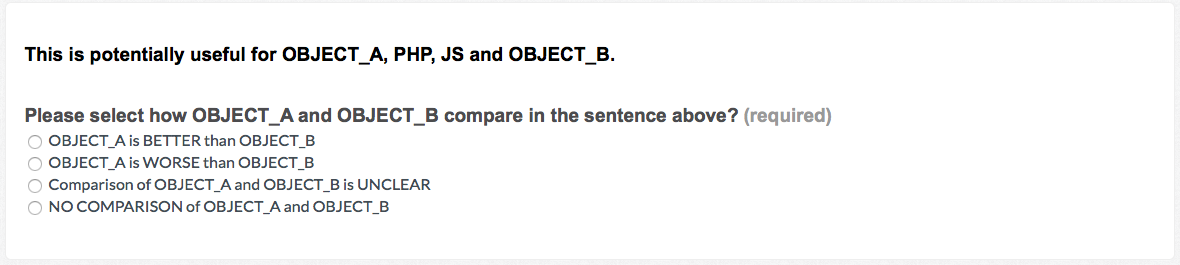
\includegraphics[width=1\textwidth]{images/prestudy/1_question}

\end{figure}

\begin{table}[h]
\centering
\caption{The classes for the first and second prestudy. They correspond to the answers the annotator could select in figure \ref{img:1_question}}
\label{tbl:prestudyclasses-a}
\begin{tabularx}{\linewidth}{lX}

\toprule
Class & Description \\ \midrule
\texttt{BETTER} & The first object in the sentence (\texttt{OBJECT\_A}) is better than the second one (\texttt{OBJECT\_B})\\
\texttt{WORSE} & The first object is worse \\
\texttt{UNCLEAR} & Neither \texttt{BETTER} nor \texttt{WORSE} fits, but the sentence is comparative\\
\texttt{NO\_COMP} & The sentence is not comparative or the sentence is a question\\
\bottomrule
\end{tabularx}
\end{table}

In each sentence, the first object of interest was replaced with \texttt{OBJECT\_A}, while the second one was replaced with \texttt{OBJECT\_B} (see table \ref{tbl:pre_1_res}). The idea behind this was to enable the annotators to quickly see which objects should be taken into account for assigning a class. Also, they should not be biased by personal preference. For example, in sentence two of table \ref{tbl:pre_1_res}, the annotator might be confused which of the objects are of interest, yet the replacement makes it clear that he should ignore \enquote{\emph{C}} and \enquote{\emph{VB}}. 

Each annotator saw five sentences to annotate per page. He was also able to look into the annotation guidelines anytime he wanted. To filter out low-quality annotators, twelve sentences were selected as test questions. Each participant took a quiz (eight test questions) before the actual annotation process. One of the five sentences was a test question as well. The annotator had to keep an accuracy of 70\% on the test questions, otherwise he was removed from the task.

Figure \ref{fig:dist_pre_a} shows the class distribution of the annotation results. As 45  sentences are comparative, the selection procedure works satisfying.

\begin{figure}[th]
\centering
\caption{The results for the first prestudy. As 45  sentences are comparative, the selection procedure worked satisfying.}
\label{fig:dist_pre_a}
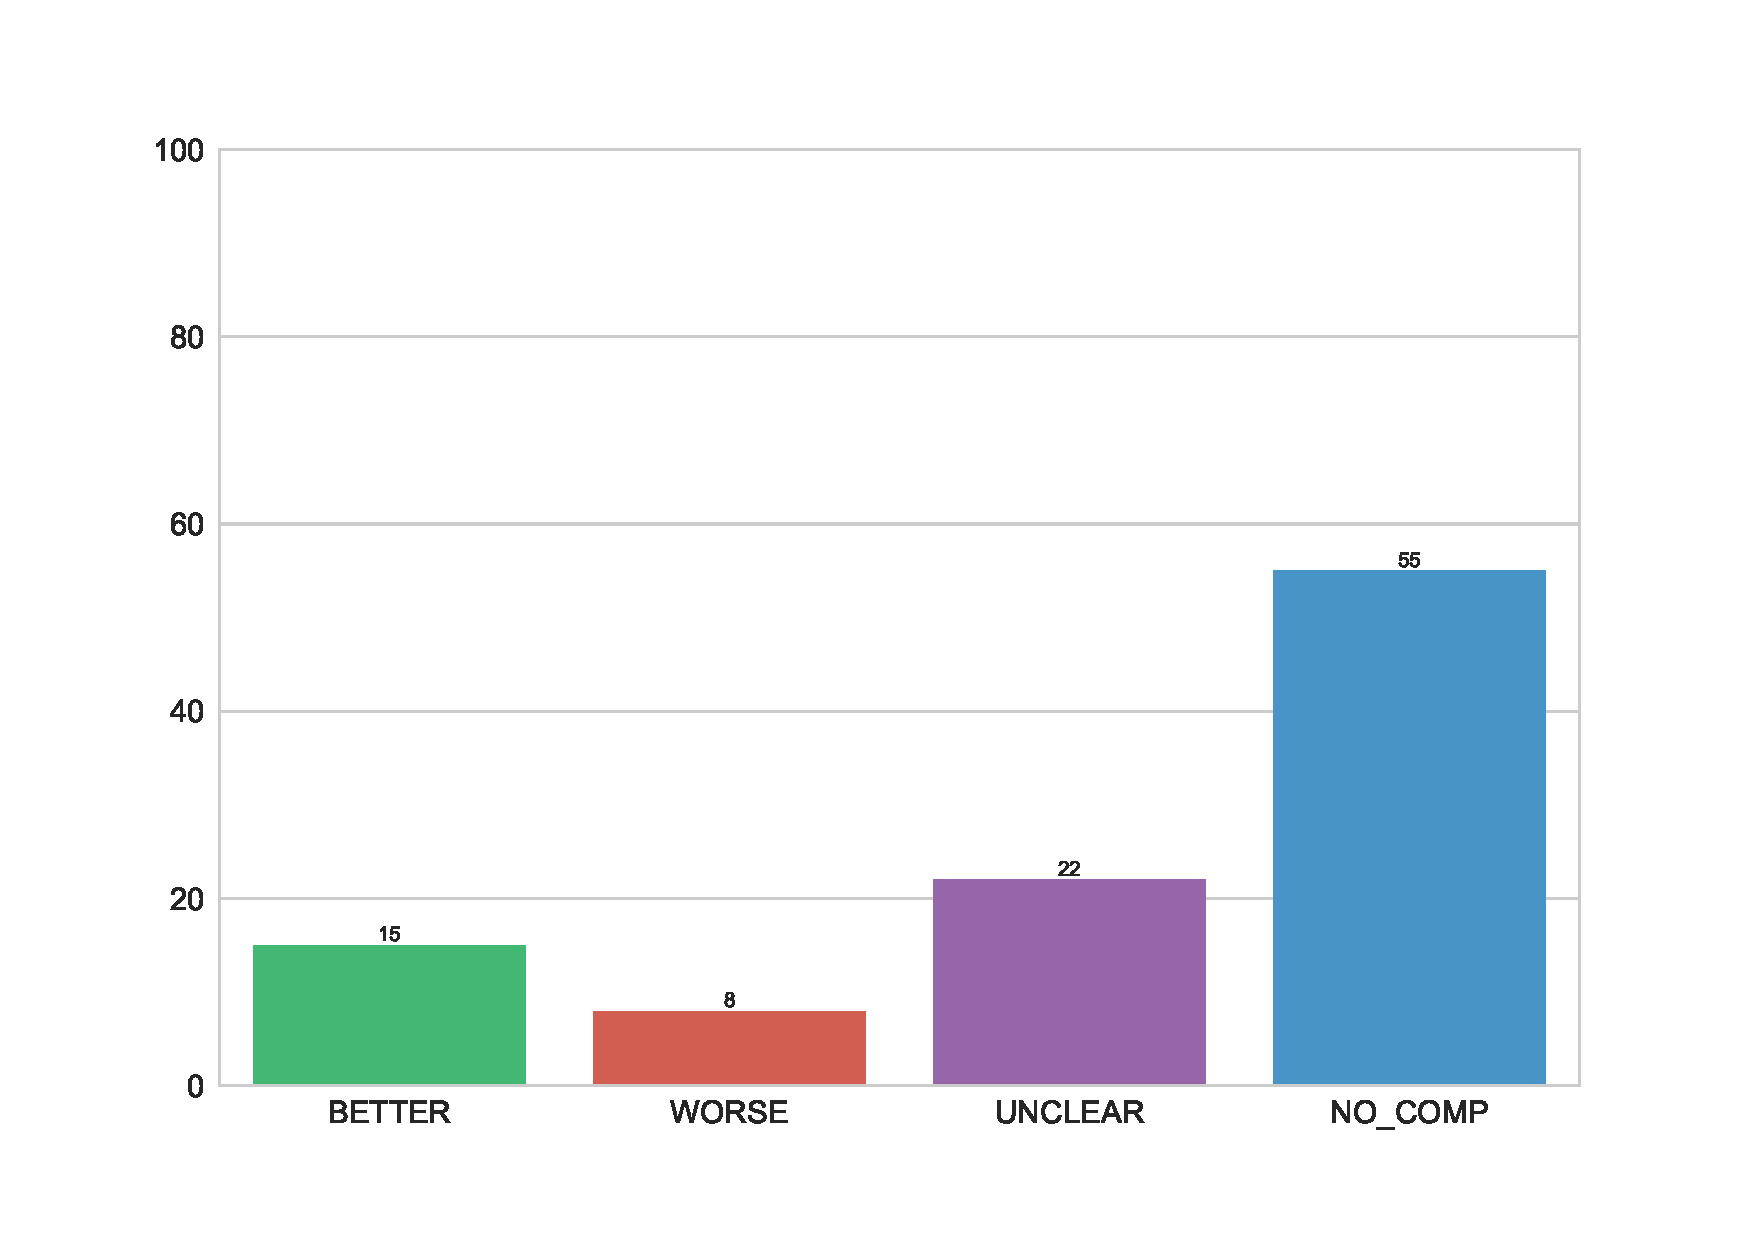
\includegraphics[width=0.8\linewidth]{images/dataset/prea-dist}
\end{figure}
\FloatBarrier

The confidence of the annotations was acceptable (see table \ref{fig:pre_a_agg}). Only for eight sentences, no class got the majority of votes. However, only thirty-seven sentences got a unanimous result.

\begin{table}[tp]
\caption{Annotation confidence for the \emph{first prestudy}. The confidence is calculated as \emph{judgments for majority class / total judgments}. Less than 51 percent confidence means no class got the majority of votes, while 100 percent means that all annotators voted for the same class.}
\label{fig:pre_a_agg}
\begin{tabularx}{\textwidth}{XXX}
\toprule
Confidence & Sentences & \% of data set \\
\midrule
100\%	&	37	&	37.00	 \\ 
91-99\%	&	0	&	0.00	 \\ 
81-90\%	&	0	&	0.00	 \\ 
71-80\%	&	5	&	5.00	 \\ 
61-70\%	&	50	&	50.00	 \\ 
51-60\%	&	0	&	0.00	 \\ 
0-50\%	&	8	&	8.00	 \\ 
\bottomrule
\end{tabularx}
\end{table}

\begin{table}[tbp]
\centering
\caption{Examples of uncertain sentences for the \emph{first prestudy}. The annotators could not agree on one class for this sentences. }
\label{tbl:pre_1_res}
\begin{tabularx}{\textwidth}{Xrrrr}
\toprule
 Sentence        & \texttt{BETTER} & \texttt{WORSE} & \texttt{UNCLEAR} & \texttt{NO\_COMP}          \\ \midrule

While \emph{OBJECT\_A} is slightly faster, \emph{OBJECT\_B} utilises memory better & 1 & 1 & 1 & 0 \\

Your C\# and VB devs can suddenly easily write web apps and your \emph{OBJECT\_A} and \emph{OBJECT\_B} devs can too - with the added bonus of much better performance. & 0 & 0 & 2 & 2 \\

The only reason \emph{OBJECT\_A} is used over \emph{OBJECT\_B}, is because of libraries.. & 0 & 1 & 1 & 1 \\

for json: i also think its better to just use \emph{OBJECT\_A}, \emph{OBJECT\_B}, perl and transform it & 1 & 0 & 1 & 1 \\

\bottomrule                              
\end{tabularx}
\end{table}


Some uncertain sentences are shown in table \ref{tbl:pre_1_res}, which displays the sentence and number of decisions per class. As one can see in sentence two, annotators often were not able to distinguish between \texttt{NO\_COMP} and \texttt{UNCLEAR}. This is true for the majority of cases were more than one classes was assigned.



Fourteen out of fifty-five participants took part in an exit survey to rate the task. The overall satisfaction was rated with 3.2 out of 5. While the instructions (4.5), difficulty (4.4) and payment (3.8) got acceptable to good ratings, the test questions (2.9) were critizied. Also, thirty-two of eighty-five potential annotators failed the quiz. A second prestudy was conducted to adress the discovered problems.


\FloatBarrier
\subsection{Second Prestudy}
Two-hundred sentences were annotated in the second prestudy. To address the shortcomings mentioned above, the task design was changed in several aspects.

However, some aspects were identical to the first study. As the sentence selection process worked fine, the same 1000 base sentences were used in the second prestudy.  Each sentence was annotated by three annotators. The annotators saw five sentences per batch, one being a test question. They had to pass a quiz of eight test questions and had to keep an accuracy of 70\% on the test questions during the annotation procedure. The classes were the same as in the first prestudy (see table \ref{tbl:prestudyclasses-a}).

As the pair \enquote{\emph{Ruby vs. Python}} requires knowledge in computer science, this need was expressed in the title of the task.
To address the problem with the confusion between \texttt{UNCLEAR} and \texttt{NO\_COMP}, the wording on this classes in the annotator's view was changed. The new view is displayed in figure \ref{img:2_question}. 

\begin{figure}[h]
\centering
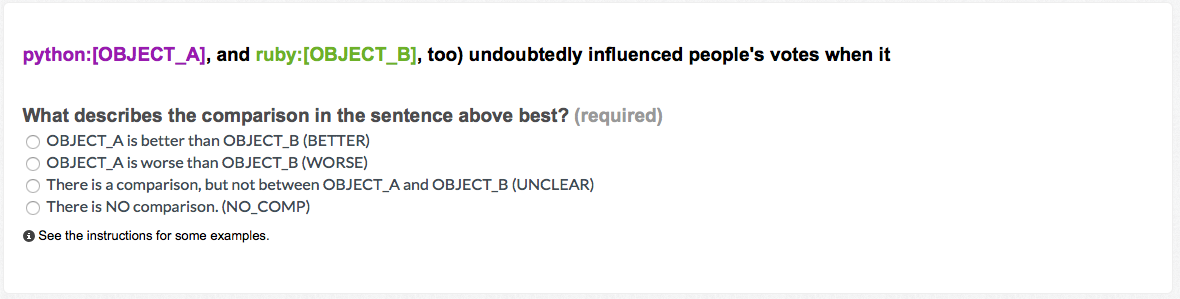
\includegraphics[width=1\textwidth]{images/prestudy/2_question}

\caption{The new annotator view for the second prestudy. The objects are now highlighted by colour.}
\label{img:2_question}
\end{figure}

In the first prestudy, some annotators complained that the test questions were not fair. In fact, they contained some special cases in a way that they did not represent the whole data set appropriatly. In the second prestudy, more test questions (fifty-one instead of twelve) test questions were used. Those test questions covered easy and hard cases. Explanations for the harder test questions were added. The annotator saw those explanations after he failed the test question.



The sentence preprocessing was altered as well. Instead of replacing the object, \mbox{\textbf{{\color[HTML]{9A14B2}:{[}OBJECT\_A{]}}}} or \textbf{{\color[HTML]{6CB219}:{[}OBJECT\_B{]}}} was appended. The colon and square brackets emphasize where the object of interest ends and the suffix begins. The idea behind this was that the removal of the objects also removed some context from the sentences, which might be useful to classify them correctly. In addition, the objects were shown in a different colour than the rest of the text.\newline



The class distribution for the two-hundred sentences is presentend in figure \ref{fig:dist_pre_b}.  As in the first prestudy, a sufficient amount of the sentences are comparative. The confidence of the annotations (see table \ref{tbl:pre_b_agg}) was better than in the first prestudy. The confusion between \texttt{UNCLEAR} and \texttt{NO\_COMP} is still the main problem. Compared to the first prestudy, the amount of sentences where all annotators agreed on one class increased from 37\% to 62\%. Table \ref{tbl:pre_2_res} shows some of the uncertain sentences.


\begin{figure}[tb]
% aktuelle zahlen 29.3; neue methode
\centering
\caption{Class Distribution for the second prestudy.}
\label{fig:dist_pre_b}
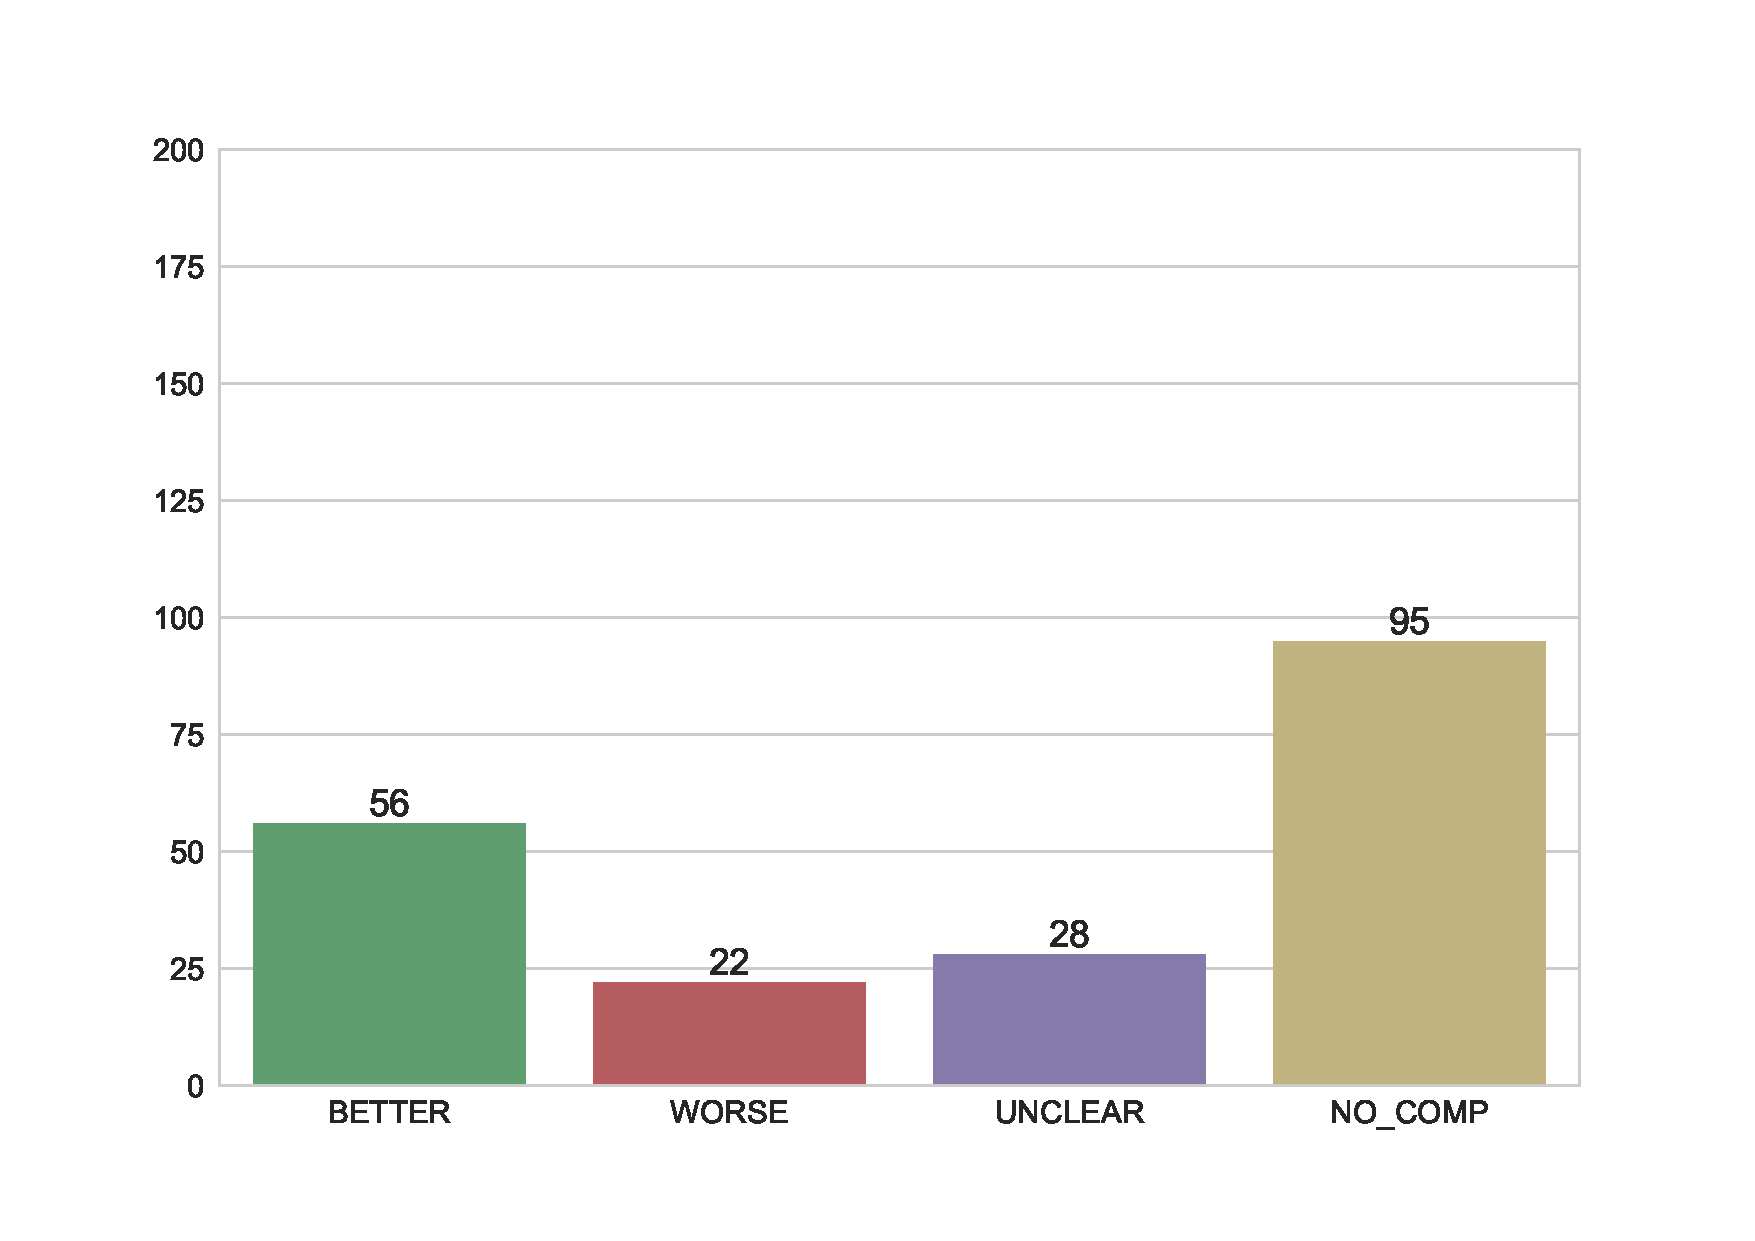
\includegraphics[width=0.8\linewidth]{images/dataset/preb-dist}
\end{figure}


\begin{table}[tp]
% aktuelle zahlen 29.3; neue methode
\caption{Annotation confidence for the \emph{second prestudy}. The confidence is calculated as \emph{judgments for majority class / total judgments}.}
\label{tbl:pre_b_agg}
\begin{tabularx}{\textwidth}{XXX}
\toprule
Confidence & Sentences & \% of data set \\
\midrule
100\%	&	124	&	62.00	 \\ 
91-99\%	&	2	&	1.00	 \\ 
81-90\%	&	2	&	1.00	 \\ 
71-80\%	&	5	&	2.50	 \\ 
61-70\%	&	57	&	28.50	 \\ 
51-60\%	&	2	&	1.00	 \\ 
0-50\%	&	8	&	4.00	 \\ 
\bottomrule
\end{tabularx}
\end{table}



\begin{table}[tp]
% aktuelle zahlen 29.3; neue methode
\centering
\caption{Examples of uncertain sentences for prestudy B. The annotators could not agree on one class for this sentences. }
\label{tbl:pre_2_res}
\begin{tabularx}{\textwidth}{Xrrrr}
\toprule
 Sentence        & \texttt{BETTER} & \texttt{WORSE} & \texttt{UNCLEAR} & \texttt{NO\_COMP}          \\ \midrule
\textbf{{\color[HTML]{9A14B2}Ruby:{[}OBJECT\_A{]}}} and \textbf{{\color[HTML]{6CB219} Python:{[}OBJECT\_B{]}}} perform significantly better. & 0 & 0 & 2 & 2 \\

Unfortunately, when it comes to potential projects \textbf{{\color[HTML]{9A14B2}Ruby:{[}OBJECT\_A{]}}} suffers because it's similarity to \textbf{{\color[HTML]{6CB219} Python:{[}OBJECT\_B{]}}} & 1 & 2 & 1 & 0 \\


Not to mention that the \textbf{{\color[HTML]{9A14B2}iPhone:{[}OBJECT\_A{]}}} and \textbf{{\color[HTML]{6CB219} Android:{[}OBJECT\_B{]}}} phones deliver a far superior user experience overall & 1 & 0 & 1 & 1 \\

Google shouldn't have mandated an inferior map app on the \textbf{{\color[HTML]{9A14B2}iPhone:{[}OBJECT\_A{]}}} (as opposed to \textbf{{\color[HTML]{6CB219} Android:{[}OBJECT\_B{]}}}). & 1 & 1 & 0 & 1 \\



\bottomrule                              
\end{tabularx}
\end{table}

 \FloatBarrier
From 125 candidate annotators, thirty-five failed the initial quiz. Twelve annotators were removed during the annotation process as they answered too many test questions wrong.

Twenty-two annotators took the exit survey. The overall satisfaction increased to 3.7 out of 5. The test question fairness was now rated with 3.7  instead of 2.9. The rating for the payment slightly increased to 3.9, yet the payment was not changed. However, the rating for the instructions decreased to 3.9 and for the difficulty to 3.5.
The change in numbers is explained by the increased amount of sentences, which introduce new cases which are not directly reflected in the annotation guidelines.

\subsection{Validation of results}
Only a small fraction of the annotators took the exit surveys in both prestudies which reduces their explanatory power. However, it gave valuable hints to improve the study design. Yet, the increased confidence of the annotations is the more important signal.

Using two comparable objects and cue words to query the index returns a satisfiying amount of comparative sentences. The changes in the second prestudy were well recieved by the annotators. In the end, they improved the quality of results as there are more cases where all annotators agreed on one class.


The distinction between \texttt{UNCLEAR} and \texttt{NO\_COMP} is still a problem. This illustrates that the choice of a class is subjective to some degree. 

Due to an error in the creation of the crowdsourcing task, the sentences where not shuffled. This means that the first one-hundred sentences of the second prestudy are the same as the one-hundred sentences of the first prestudy. Another problem is the bias: all sentences contained only the pairs \emph{Ruby vs. Python} and \emph{Android vs. iPhone}. Because the goal of the prestudy was mainly to assess the sentence selection method and the guidelines, this does not invalidate the results. Those problems were removed in the main study.
\hfill\newline

All in all, the prestudy was successful. There are only few cases where no agreement on the class could be achieved. The prestudy showed that the task at hand is not easy, but feasable.

\newpage
\section{Main Study}
\label{sec:mainstudy}
\subsection{Design changes}
\label{sec:designchanges}
The insights from the prestudy influcenced the design of the main study.

The definition of classes changed (table \ref{tbl:mainstudy-classes}). \texttt{UNCLEAR} was renamed to \texttt{OTHER}, \texttt{NO\_COMP} to \texttt{NONE}. Those names are a better description for the classes. Eventually, after the first 2250 sentences were finished the class \texttt{OTHER} was dropped completly (see section \ref{sec:brands}). The change was reflected in the annotation guidelines as well. 

\begin{table}[h]
\centering
\caption{The final classes for the main study.}
\label{tbl:mainstudy-classes}
\begin{tabular}{@{}ll@{}}
\toprule
Class & Description \\ \midrule
\texttt{BETTER} & The first object in the sentence is better than the second object\\
\texttt{WORSE} & The first object is worse \\
\texttt{NONE} & Neither better nor worse fit\\
\bottomrule
\end{tabular}
\end{table}

Instead of one big task, several tasks per domain were created. All tasks used the same annotation guidelines. Each sentence was at least annotated by five annotators.


\subsection{Sentence Selection}
The sentence selection process was similar to the prestudy. The pairs and the cue words (see figure \ref{fig:cue_words}) changed. The cue words were generated using JoBimText, a software package for distributional semantics. JoBimText\footnote{http://ltmaggie.informatik.uni-hamburg.de/jobimviz/ (28.02.2018)} was queried for the nine words most similar to \emph{better} and \emph{worse}, so that more, different comparisons are captured by the selection process.

\begin{figure}[hb]
\centering
\caption{Cue words. It is expected that those words appear frequently in comparative sentences.}
\label{fig:cue_words}
\begin{multicols}{4}
better

easier

faster

nicer

wiser

cooler

decent

safer

superior

solid

terrific

worse

harder

slower

poorly

uglier

poorer

lousy

nastier

inferior

mediocre
\end{multicols}
\end{figure}

Three domains were selected for the object pairs. The domains were chosen in a way that a majority of people can decide whether a sentence contains a comparison or not. Also, a wide range of comparison patterns should be included in the data.

The most specific domain was \enquote{\emph{Computer Science Concepts}}. It contained objects like programming languages, database products and technology standards such as Bluetooth and Ethernet.  Many computer science concepts can be compared objectively. For instance, one can compare Bluetooth and Ethernet on their transmission speed. Some basic knowledge of computer science was needed to label sentences correctly: to compare Eclipse and NetBeans, the annotator must know what an Integrated Development Environment (IDE) is and that both objects are Java IDEs.  The need for this knowledge was communicated to the prospective annotators. The objects for this domain were manually extracted from \enquote{\emph{List of ...}} articles from Wikipedia\footnote{ADD TO APPENDIX}.

The second, broader domain was \enquote{\emph{Brands}}. It contains objects of different types (e.g. car brands, electronics brands, and food brands). As brands are present in everyday life of people, it is expected that anyone can label the majority of sentences containing well known brands such as \enquote{\emph{Coca-Cola}} or \enquote{\emph{Mercedes}}. As with computer science, the objects for this domain were extracted from \enquote{\emph{List of ...}} articles from Wikipedia\footnote{ADD TO APPENDIX}.

The last domain is not restricted to any topic. For each one of twenty-four randomly selected seed words, ten similar words were extracted using JoBimText. The seed words (see figure \ref{fig:seed}) were created using randomlists.com\footnote{https://randomlists.com  (checked: 25.01.2018)}. Listing \ref{lst:jbtres} shows the result\footnote{http://ltmaggie.informatik.uni-hamburg.de/jobimviz/ws/api/stanford/jo/similar/harvard\%23NP?numberOfEntries=10&format=json (25.01.2018); Some uninteresting fields were removed for brevity} for the seed word \enquote{\emph{Yale}}. Duplicates or too broad terms (like \emph{university}) were removed by manually.

\begin{figure}[bth]
\centering
\caption{Seed words. The words were used to create pseudo-random pairs for the \emph{Random} domain. }
\label{fig:seed}
\begin{multicols}{5}
book%23NN

car%23NN

carpenter%23NN

cellphone%23NN

christmas%23NN

coffee%23NN

cork%23NN

florida%23NP

hamster%23NN

hiking

hoover%23NP

metallica%23NP

nbc%23NP

netflix%23NP

ninja%23NN

pencil%23NN

salad%23NN

soccer%23NN

starbucks%23NN

sword%23NN

tolkien%23NP

wine%23NN

wood%23NN

xbox%23NP

yale%23NP
\end{multicols}

\end{figure}

\begin{minipage}{\linewidth}
\begin{lstlisting}[language=json,label=lst:jbtres,caption=JoBimTexts response. Shows similar words to \emph{\enquote{Yale}}. Those objects can be compared meaningful.]
[...]
   "results":
      [{"score":701.0,"key":"yale#NP"},
      {"score":245.0,"key":"harvard#NP"},
      {"score":151.0,"key":"princeton#NP"},
      {"score":135.0,"key":"mit#NP"},
      {"score":135.0,"key":"cornell#NP"},
      {"score":121.0,"key":"stanford#NP"},
      {"score":116.0,"key":"university#NP"},
      {"score":111.0,"key":"nyu#NP"},
      {"score":111.0,"key":"university#NN"},
      {"score":109.0,"key":"dartmouth#NP"}]
\end{lstlisting}
\end{minipage}

In the following, this domain is called \emph{Random}. Some example pairs for all domains are shown in table \ref{tbl:exp_pairs}.
\begin{table}[h]
\centering
\caption{Examples of objects pairs for the main study. Those pairs were used to extract sentences from the ElasticSearch index.}
\label{tbl:exp_pairs}

\begin{tabularx}{\textwidth}{XXX}
\toprule
Brands & Computer Science & Random \\
\midrule
Microsoft vs. Apple & Java vs. Python & Baseball vs. Hockey \\
Nikon vs. Leica & Eclipse vs. Netbeans & Fishing vs. Swimming\\
Coca-Cola vs. Pepsi & OpenGL vs. Direct3D & SUV vs. Minivan\\
Nike vs. Adidas & Integer vs. Float & Kennedy vs. Nixon\\
Ibuprofen vs. Advil & USB vs. Bluetooth & Plastic vs. Wood\\
Ford vs. Honda & Oracle vs. MysQL & Harvard vs. Princeton\\

\bottomrule

\end{tabularx}

\end{table}

Especially for brands and computer science, the object lists were long (4493 brands and 1339 for computer science). The frequency of each object was checked using a frequency dictionary to reduce the number of possible pairs. All objects with a frequency of zero and ambiguous objects were removed from the list. For instance, the objects \enquote{\emph{RAID}} (a hardware concept) and \enquote{\emph{Unity}}  (a game engine) were removed from the computer science list as they are also regularly used nouns.

The remaining objects were combined to pairs. For each type, all possible combinations were created. For brands and computer science, the type is the URL of the Wikipedia page. For the random domain, the seed word was used. This procedure guarantees that only meaningful pairs are created.




The index was then queried for entries containing both objects of each pair. For 90\% of the queries, the cue words were added to the query. All pairs were the query yielded at least one-hundred sentences were kept.

From all sentences of those pairs, 2500 for each category were randomly sampled as candidates for the crowdsourcing task. To check the sentence selection method once again, a small, random subset of the sentences was labelled by the author prior to the crowdsourcing task. Those labels were discarded for the crowdsourcing task.
The label distribution of the 742 sentences is presented in the figure \ref{fig:sample}. As the numbers are similar to the prestudy, the procedure is still valid.


\begin{figure}[h]
\centering
\caption{Result of 742 manually labelled sentences. The labelling was done to see what result can be expected from the crowdsourcing task and if the sentence sampling method still works.}
\label{fig:sample}
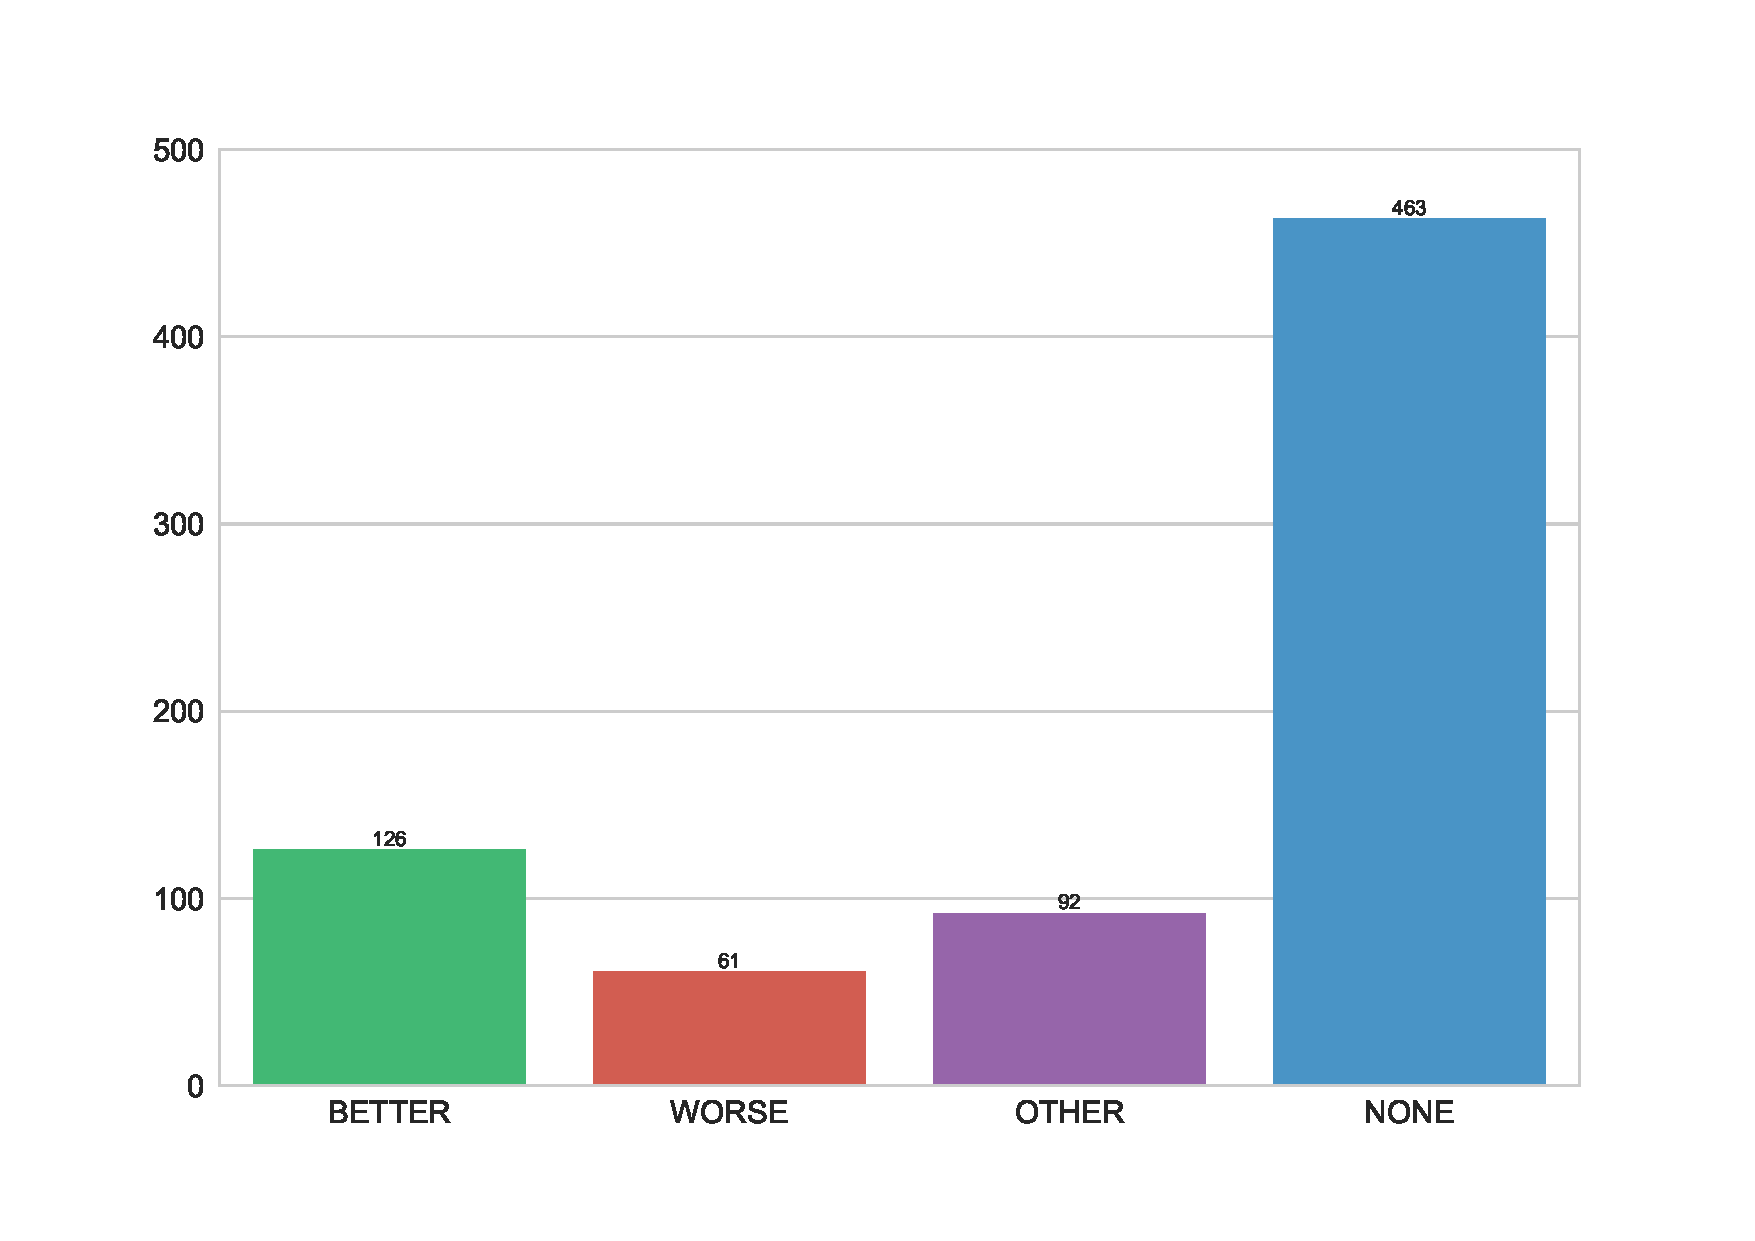
\includegraphics[width=0.8\linewidth]{images/dataset/pre-dist}
\end{figure}
\FloatBarrier
\subsection{Brands}
\label{sec:brands}

% zahlen 23.3
For the Brands domain, 2335 sentences were annotated. The sentences contained objects of sixty-three pairs. As shown in table \ref{fig:brand_agg}, the annotators could agree on one class for the majority of sentences.


% zahlen 29.3
\begin{table}[h]
\caption{Annotation confidence for the domain \emph{Brands}. The confidence is calculated as \emph{judgments for majority class / total judgments}.}
\label{fig:brand_agg}
\begin{tabularx}{\textwidth}{XXX}
\toprule
Confidence & Sentences & \% of data set \\
\midrule
100\%	&	1719	&	71.30	 \\ 
91-99\%	&	0	&	0.00	 \\ 
81-90\%	&	34	&	1.41	 \\ 
71-80\%	&	337	&	13.98	 \\ 
61-70\%	&	8	&	0.33	 \\ 
51-60\%	&	256	&	10.62	 \\ 
0-50\%	&	57	&	2.36	 \\ 
\bottomrule
\end{tabularx}
\end{table}



The class distribution is presented in figure \ref{fig:brands_fin}. The amount of comparative sentences is lower (24.45\%) than in the prestudy. The reason for this is seen in the abandonment of the \texttt{OTHER} (\texttt{UNCLEAR}) class. 

% zahlen 29.3
\begin{figure}[h]
\centering
\caption{Class distribution for sentences of the domain \emph{Brands}}
\label{fig:brands_fin}
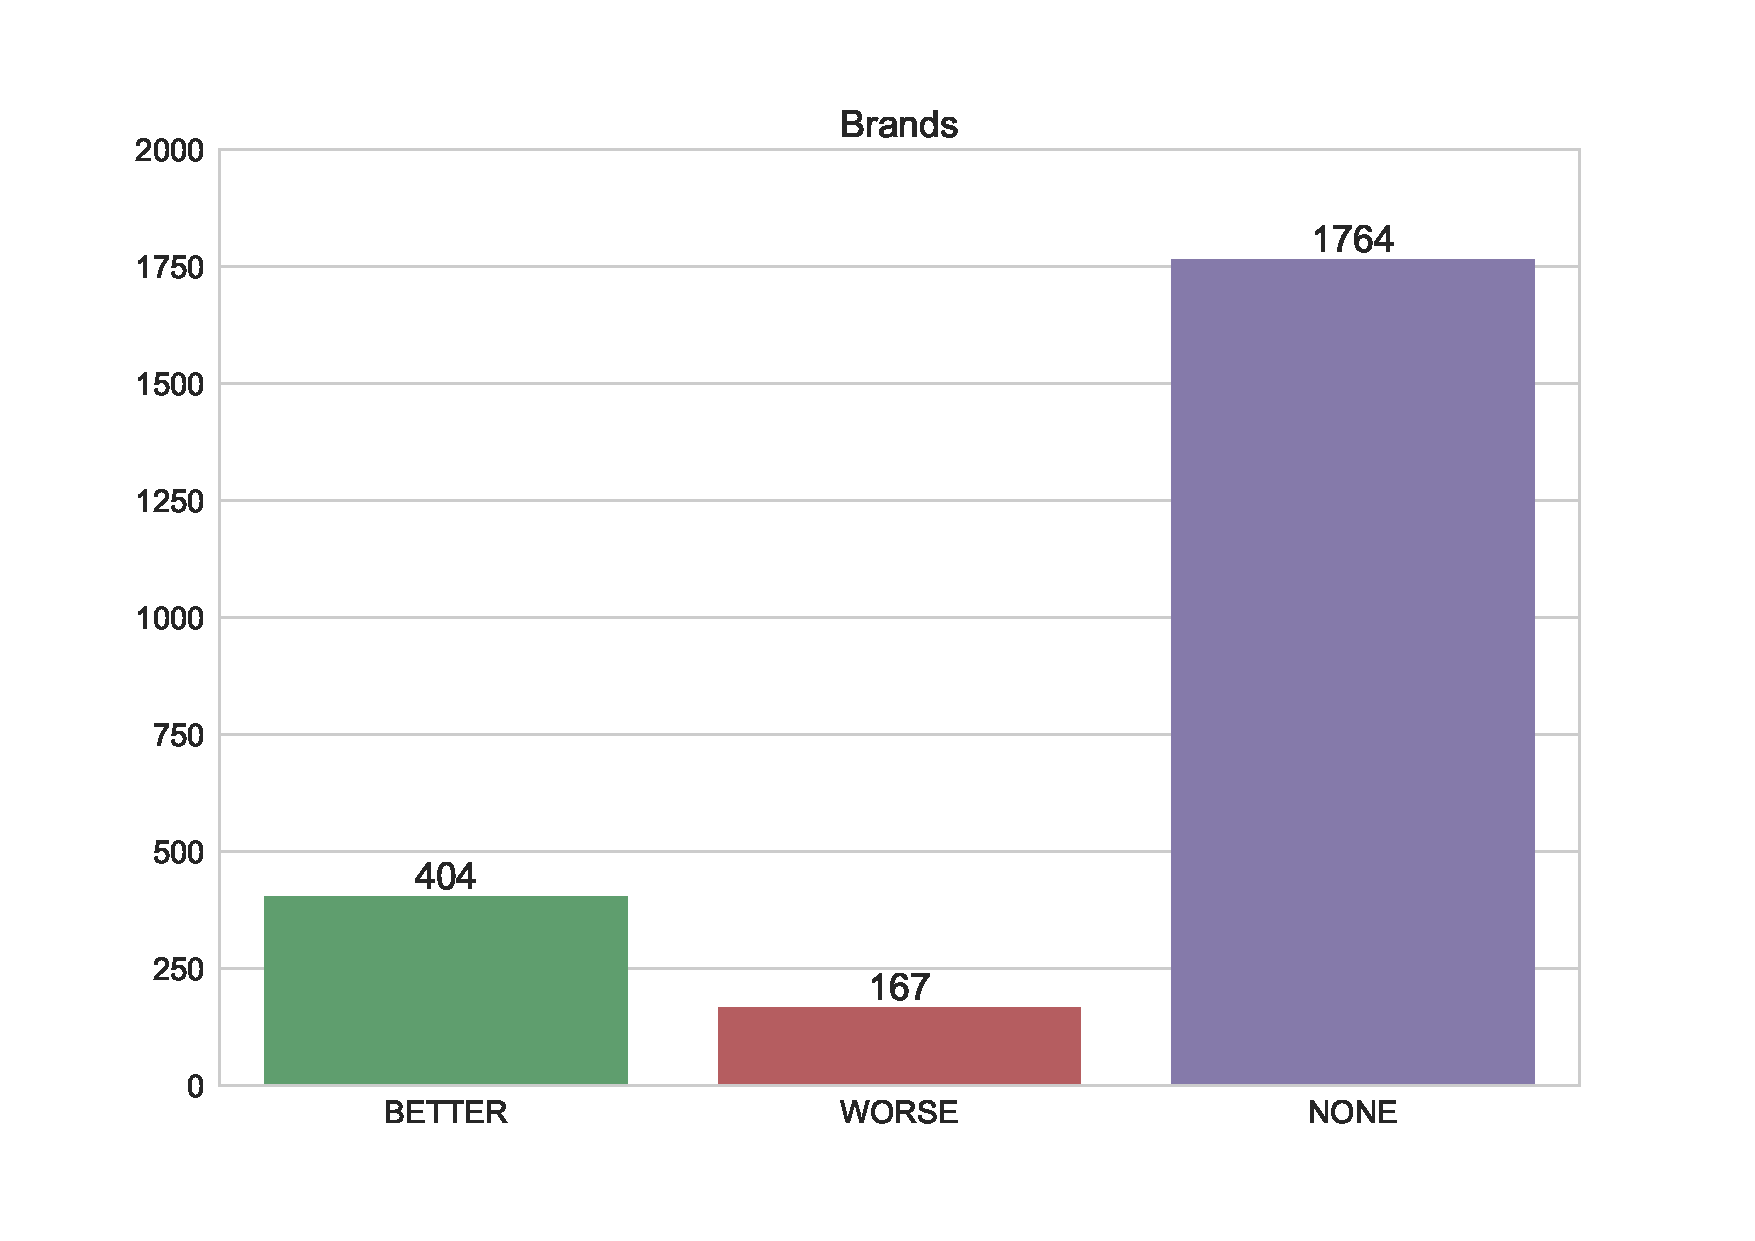
\includegraphics[width=0.8\textwidth]{images/dataset/Brands-dist}
\end{figure}




% zahlen alt
Even with the rephrasing of \texttt{UNCLEAR} to \texttt{OTHER}, it was too confusing for the annotators. The class was not different enough from \texttt{NONE} (\texttt{NO\_COMP}). Eventually, all sentences labelled as \texttt{OTHER} (124 sentences for brands) were merged into \texttt{NONE}. This decision was made after 750 sentences were labelled for each domain. First machine learning experiments also showed that \texttt{OTHER} is not distinguishable from \texttt{NONE} for all tested features and algorithms.

For the first 750 sentences (with four classes), 47\% failed the initial quiz (357 out of 755). During the annotation process, 13\% answered to many test questions wrong. The numbers improved after the class \texttt{OTHER} was removed: only 25\% failed the initial quiz and 8\% were removed during the annotation process.

150 annotators took the exit survey to rate the task on a scala from one to five. Overall, the task was rated with 3.7. The instructions got 4.0, the fairness of test questions 3.5, the difficulty 3.6 and the payment 3.7.\footnote{The numbers are the average of the survey results for each task created on CrowdFlower, weighted by the number of participants. The results for each task can be found in the appendix.} Broken down, the four-class task (67 participants) got a rating of 3.5, the three-class task (83 participants) 3.8.


\subsection{Computer Science}
% zahlen 23.3
For the Computer Science domain, 2425 sentences (containing one of fourty-two pairs) were annotated. As with brands, the confidence of the annotations (table \ref{fig:compsci_agg}) is satisfactory. The class distribution (figure \ref{fig:compsci_fin}) is better, as more sentences are comparative.

\begin{table}[h]
\caption{Annotation confidence for the domain \emph{Computer Science}. The confidence is calculated as \emph{judgments for majority class / total judgments}. }
\label{fig:compsci_agg}
\begin{tabularx}{\textwidth}{XXX}
\toprule
Confidence & Sentences & \% of data set \\
\midrule
100\%	&	1698	&	70.02	 \\ 
91-99\%	&	0	&	0.00	 \\ 
81-90\%	&	25	&	1.03	 \\ 
71-80\%	&	369	&	15.22	 \\ 
61-70\%	&	18	&	0.74	 \\ 
51-60\%	&	246	&	10.14	 \\ 
0-50\%	&	69	&	2.85	 \\ 
\bottomrule
\end{tabularx}
\end{table}
% zahlen 23.3

\begin{figure}[h]
\centering
\caption{Class distribution for sentences of the domain \emph{Computer Science}}
\label{fig:compsci_fin}
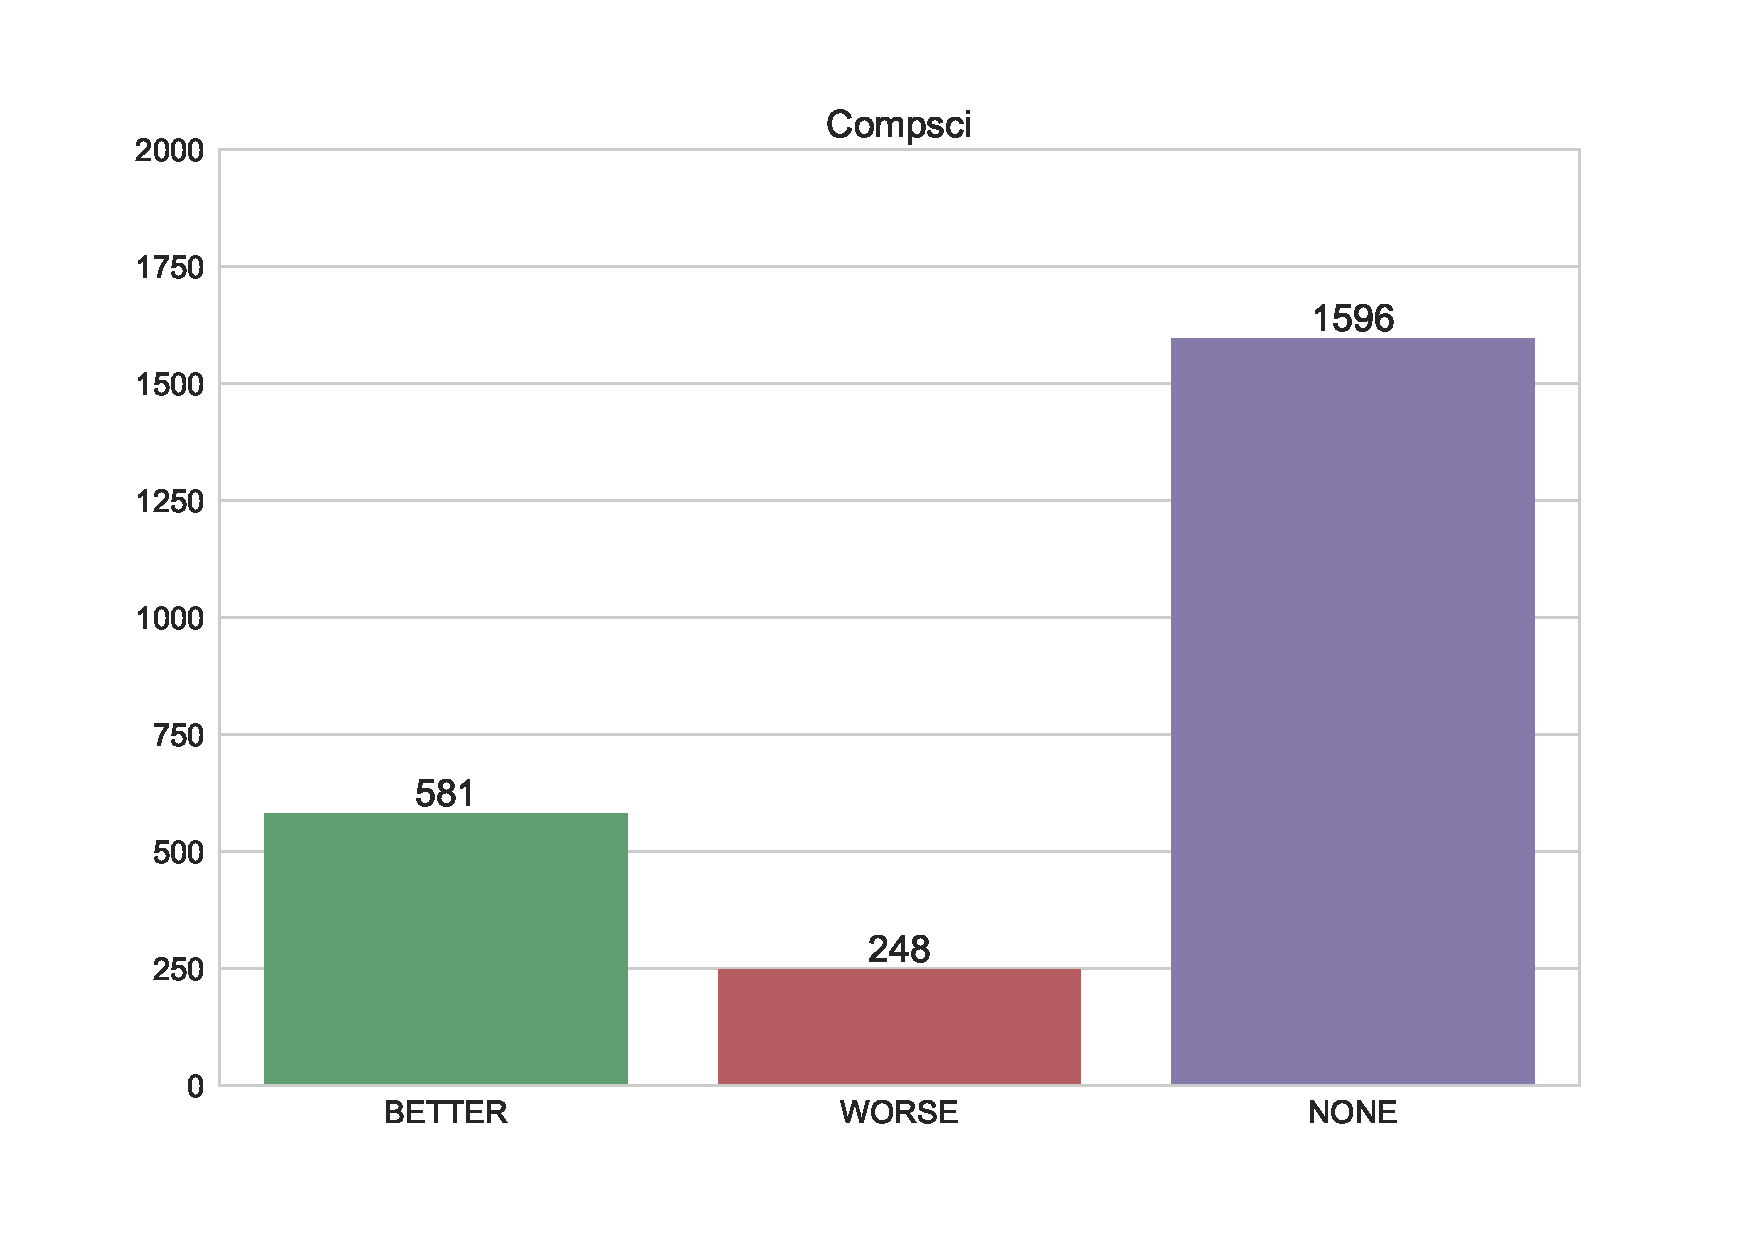
\includegraphics[width=0.8\textwidth]{images/dataset/Compsci-dist}
\end{figure}

% zahlen neu
As with Brands, 48\% failed the initial quiz for the task with four classes. 25\% dropped out during the annotation process. Again, the numbers improved after \texttt{OTHER} was removed. Only 15\% failed the quiz and 7\% were removed during the annotation process.

106 annotators took the exit survey. The task was rated with 3.9. The instructions (the instructions were the same for all tasks) got 4.2, test question fairness 4.1, difficulty 3.9 and payment (all tasks had the same payment) 3.9 as well. The four-class task (27 participants) got a rating of 3.5, the three-class task (79 participants) 3.9.
\subsection{Random}
The random domain has 2439 sentences and 167 pairs. The confidence values (table \ref{fig:random_agg}) and class distribution (figure \ref{fig:random_fin}) are satisfactory.
   % zahlen 23.3 
\begin{table}[h]
\caption{Annotation confidence for the domain \emph{Random}. The confidence is calculated as \emph{judgments for majority class / total judgments}.}
\label{fig:random_agg}
\begin{tabularx}{\textwidth}{XXX}
\toprule
Confidence & Sentences & \% of data set \\
\midrule
100\%	&	1753	&	71.87	 \\ 
91-99\%	&	0	&	0.00	 \\ 
81-90\%	&	16	&	0.66	 \\ 
71-80\%	&	362	&	14.84	 \\ 
61-70\%	&	7	&	0.29	 \\ 
51-60\%	&	252	&	10.33	 \\ 
0-50\%	&	49	&	2.01	 \\ 
\bottomrule
\end{tabularx}
\end{table}


\begin{figure}[h]
\centering
\caption{Class distribution for sentences of the domain \emph{Random}}
\label{fig:random_fin}
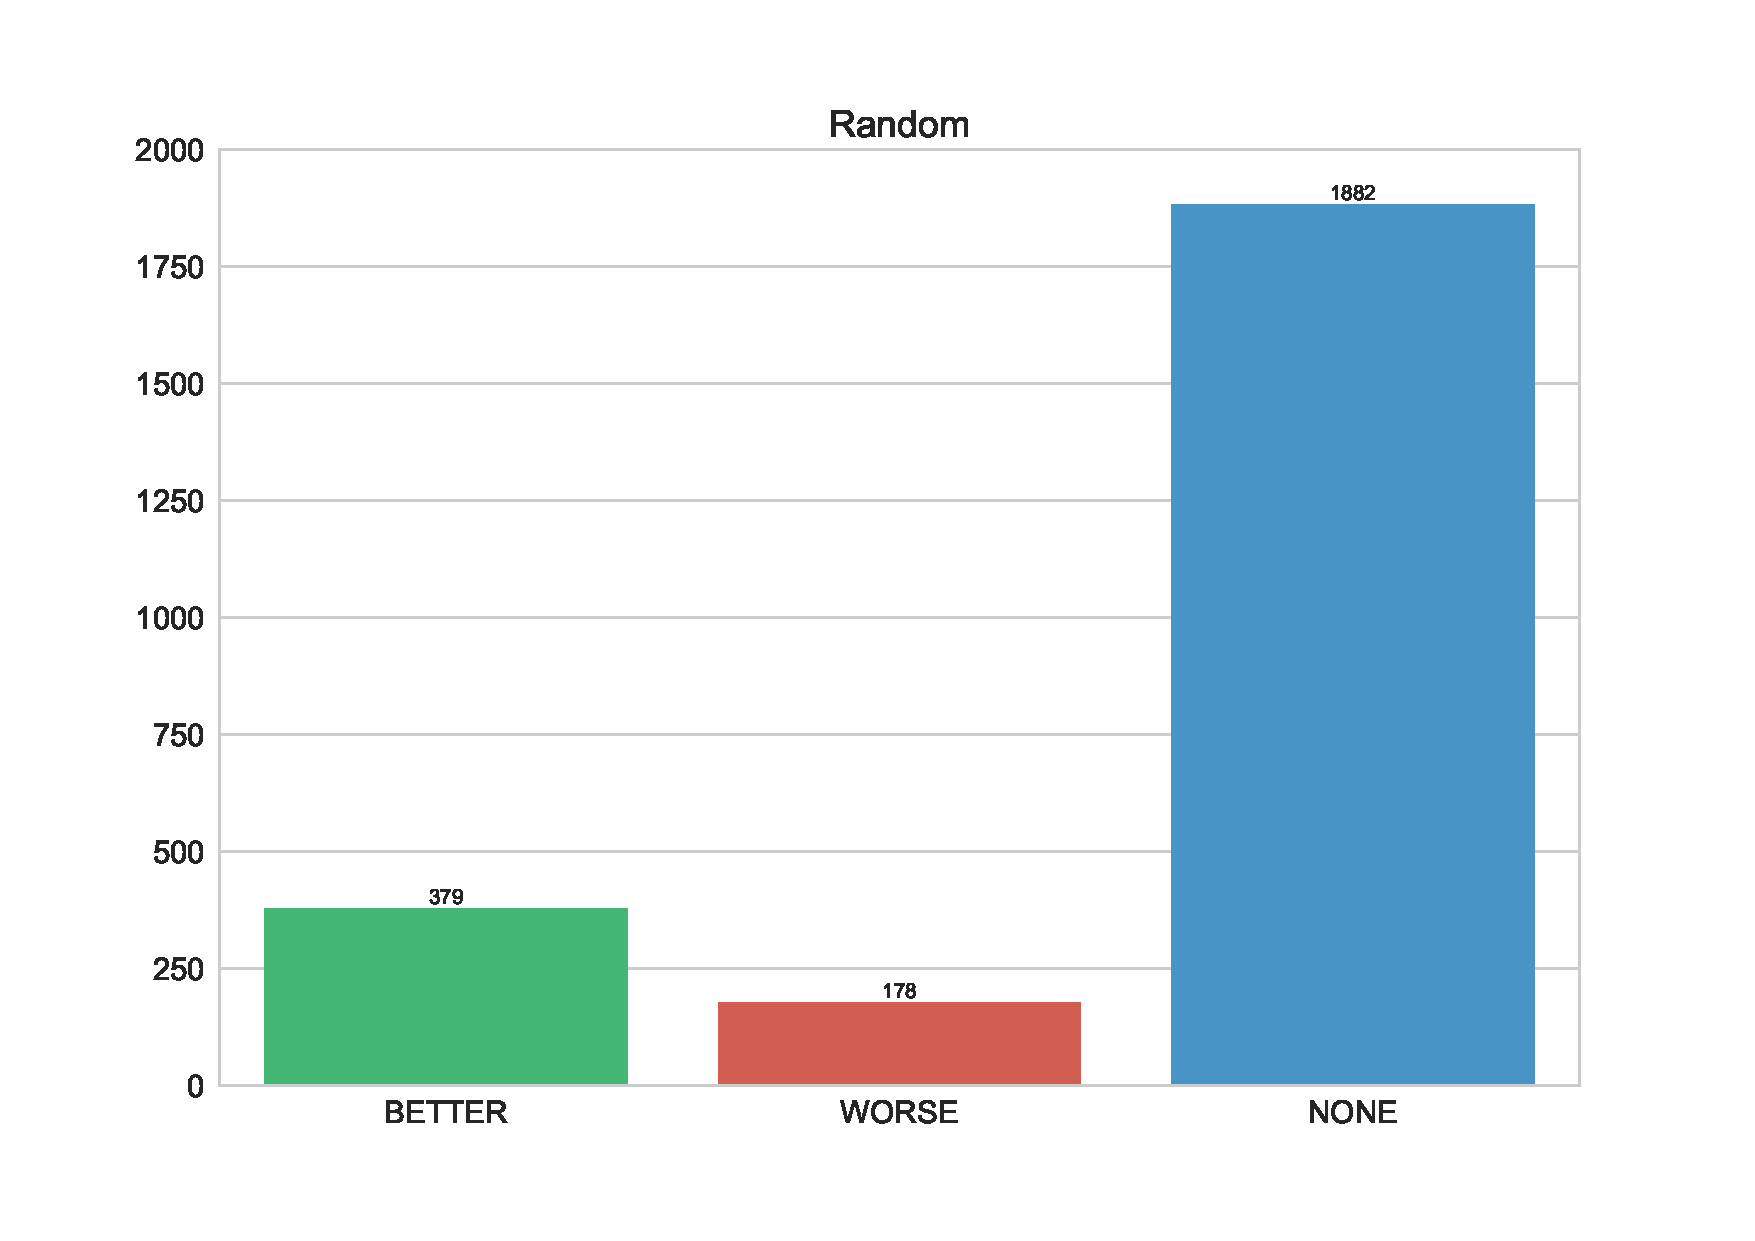
\includegraphics[width=0.8\textwidth]{images/dataset/Random-dist}
\end{figure}


As with the other domains, the first 750 sentences (with \texttt{OTHER}) performed worse than the rest: 44\% dropped out during the quiz, 16\% were removed during the annotation process. For the three-class task, the numbers improved to 14\% (quiz) and 7\% (annotation task).

97 participants rated the task with 3.6 (four classes: 3.1, 29 participants; three classes: 3.9, 68 participants). The instructions got 4.0, test question fairness 3.8, difficulty of the task 3.8 and payment 3.5.


\subsection{Validation of results}
% zahlen 23.3
Table \ref{fig:all_agg} summarises the confidence of the annotations on all three domains. The annotators could agree on one class for the majority of the sentences. Only for 169 sentences (2.35\%), no class got the majority of votes. 

\begin{table}[hp]
\caption{Annotation confidence for all domains. The confidence is calculated as \emph{judgments for majority class / total judgments}.}
\label{fig:all_agg}
\begin{tabularx}{\textwidth}{XXX}
\toprule
Confidence & Sentences & \% of data set \\
\midrule
100\%	&	5111	&	71.00	 \\ 
91-99\%	&	0	&	0.00	 \\ 
81-90\%	&	75	&	1.04	 \\ 
71-80\%	&	1057	&	14.68	 \\ 
61-70\%	&	33	&	0.46	 \\ 
51-60\%	&	754	&	10.47	 \\ 
0-50\%	&	169	&	2.35	 \\ 
\bottomrule
\end{tabularx}
\end{table}

Table \ref{tbl:all_res} shows some examples on uncertain sentences. The first two sentences are comparative. Because of the missing context, a decision for one class is hard. For instance, it depends on the use case if the hardness of stone is better or worse than the hardness of metal.

It is unclear if \emph{Groovy} and \emph{Java} are compared in sentence three. On one hand, one can understand this sentence in a way \emph{Groovy} is easier than \emph{Java}. On the other hand, it can be understood in a way that \emph{Groovy} supports Java programmers.

The fourth sentence does not explicitly states that one is better than the other.
% zahlen 23.3
\begin{table}[htbp]
\centering
\caption{Examples of uncertain sentences of the main study. The annotators could not agree on one class for this sentences.}
\label{tbl:all_res}
\begin{tabularx}{\textwidth}{lXrrr}
\toprule
\# & Sentence        & \# BETTER  & \# WORSE & \# NONE            \\ \midrule
1 & Goodnight \textbf{{\color[HTML]{9A14B2}NetBeans:{[}OBJECT\_A{]}}}, Hello \textbf{{\color[HTML]{6CB219}Eclipse:{[}OBJECT\_B{]}}} & 2&2&1\\

2 & \textbf{{\color[HTML]{9A14B2}stone:{[}OBJECT\_A{]}}} is harder than \textbf{{\color[HTML]{6CB219}metal:{[}OBJECT\_B{]}}}. & 1 & 2 & 2 \\

3 & The new version of the \textbf{{\color[HTML]{9A14B2}Groovy:{[}OBJECT\_A{]}}} programming language aims to make life easier for programmers who work with \textbf{{\color[HTML]{6CB219}Java:{[}OBJECT\_B{]}}} and SQL, the language's developers note & 3 & 0 & 3 \\

4 & Even if this \textbf{{\color[HTML]{9A14B2}juice:{[}OBJECT\_A{]}}} isn't your typical \textbf{{\color[HTML]{6CB219}cider:{[}OBJECT\_B{]}}}, it's just as good if not better in our opinion! & 2 & 1 & 2 \\

5 & Only Nevada (14.4 percent), \textbf{{\color[HTML]{9A14B2}michigan:{[}OBJECT\_A{]}}}  (13 percent) and  \textbf{{\color[HTML]{6CB219}california:{[}OBJECT\_B{]}}} (12.4 percent) were worse. & 2 & 1 & 2\\
\bottomrule                              
\end{tabularx}
\end{table}


The class distribution (figure \ref{fig:all_fin}) is similar to the prestudy. As expected, the majority of sentences is not comparative. 
The class \texttt{BETTER} is more than twice as big as the class \texttt{WORSE}, which will complicate the classification.
% zahlen 23.3


\begin{figure}[htbp]
\centering
\caption{Distribution of classes in the final crowdsourcing data set.}
\label{fig:all_fin}
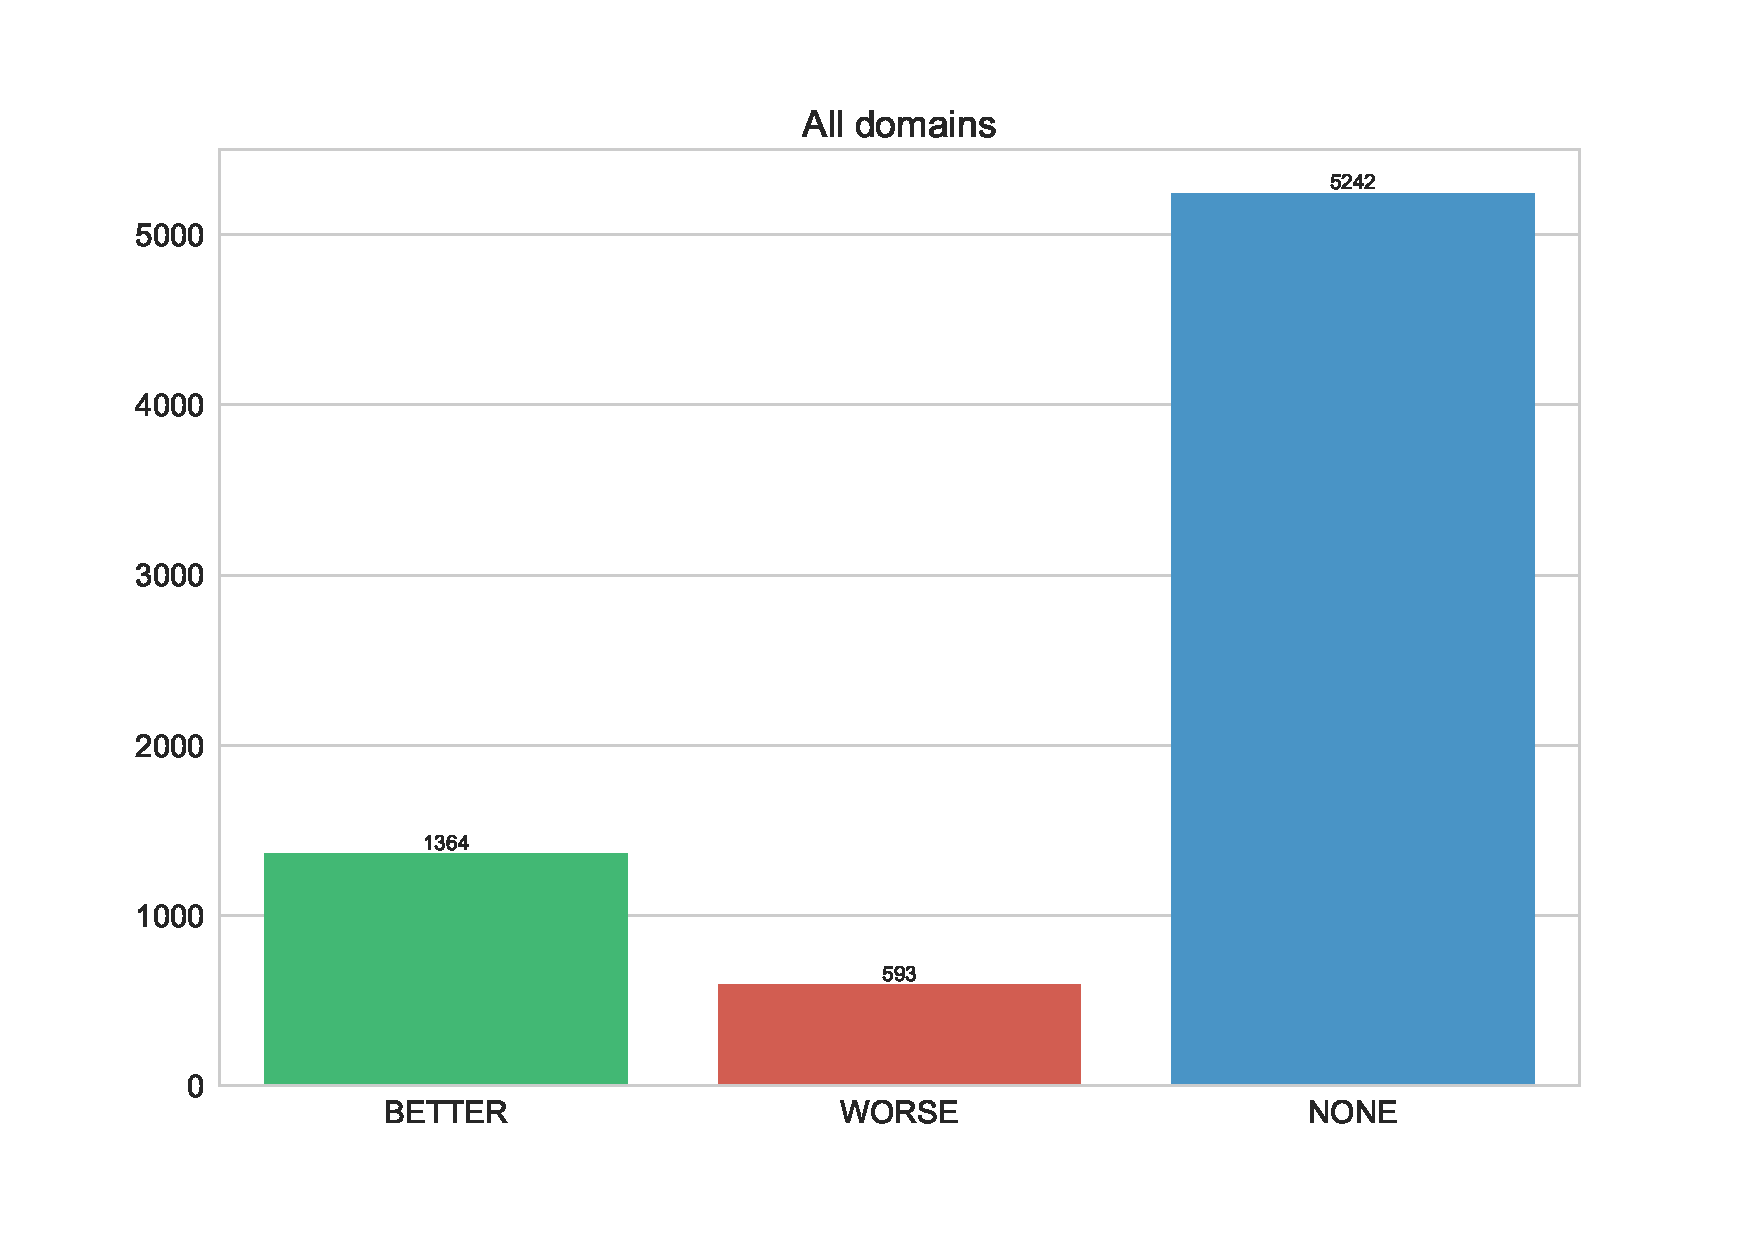
\includegraphics[width=0.8\textwidth]{images/dataset/Alldomains-dist}
\end{figure}

% zahlen 23.3
In the end, the crowdsourcing task was successful. For the majority of sentences (71.00\%) the annotators could agree on one class, while the amount of totally unclear sentences is small (2.35\%).
\FloatBarrier